%%%%%%%%%%%%%%%%%%%%%%%%%%%%%%%%%%%%%%%%%%%%%%%%%%%%%%%%%%%%%%%%%%%
% Chapter 5: Results
%%%%%%%%%%%%%%%%%%%%%%%%%%%%%%%%%%%%%%%%%%%%%%%%%%%%%%%%%%%%%%%%%%%

\chapter{Results \& Discussions}
\label{chap:result}

% khả năng là nhập ablation study vào trong 2 phần sau main

\section{Main results}

% vẽ, mô tả cái bảng tổng hợp
% Kết quả chính của công trình này được thể hiện trong bảng \ref{tab:mine_nhits}. Theo đó, phương pháp đề xuất của chúng tôi đạt hiệu quả vượt trội trên tất cả các metrics trên cả hai tập dữ liệu phi chu kỳ (\verb|USD/JPY|, \verb|multi-fx|) so với \verb|NHITS|. Trên các tập dữ liệu có chu kỳ (\verb|ETT-m2|, \verb|WTH|), mô hình của chúng tôi đạt hiệu quả gần như tương đương hoặc có phần tốt hơn so với baseline model.

The main results of this work are shown in table \ref{tab:mine_nhits}. Accordingly, our proposed method outperforms \verb|NHITS| on all metrics on both aperiodic datasets (\verb|USD/JPY|, \verb|multi-fx|). On periodic datasets (\verb|ETT-m2|, \verb|WTH|), our model performs almost the same or better than the baseline model in some cases.

\begin{table}[h]
    \centering
    \cprotect\caption{Classification results (\%) of \verb|Temporal-ML| and \verb|NHITS|. Best results per metrics are boldfaced. (\mbox{*}): Our method.}
    \label{tab:mine_nhits}
    \resizebox{\columnwidth}{!}{\begin{tabular}{c|c|cccc}
    \toprule
    \multicolumn{1}{c}{}                &                                & $accuracy$              & $precision$             & $recall$                & $F1-score$                 \\
    \hline
    \multirow{2}{*}{\Verb|USD/JPY|}     & \Verb|NHITS|                   & $58.46$                 & $58.24$                 & $57.65$                 & $55.82$            \\
                                        & \Verb|Temporal-ML|\mbox{*}     & $\mathbf{70.33\pm1.69}$ & $\mathbf{70.73\pm1.82}$ & $\mathbf{70.26\pm1.93}$ & $\mathbf{69.28\pm2.50}$    \\
                                        % & Ours(\Verb|BiLSTM+CNN|)  & $68.75\pm1.78$          & $69.15\pm1.55$          & $68.73\pm1.77$          & $69.14\pm2.17$             \\
    \hline
    \multirow{2}{*}{\Verb|multi-fx|}    & \Verb|NHITS|                   & $53.51\pm5.02$          & $53.90\pm7.68$          & $53.64\pm4.05$          & $50.20\pm7.35$              \\
                                        & \Verb|Temporal-ML|\mbox{*}     & $\mathbf{66.26\pm7.45}$ & $\mathbf{67.08\pm8.97}$ & $\mathbf{65.76\pm7.79}$ & $\mathbf{64.06\pm10.00}$   \\
                                        % & Ours(\Verb|BiLSTM+CNN|)  & $66.08\pm8.19$          & $66.56\pm9.23$          & $65.41\pm8.66$          & $63.78\pm10.83$            \\
    \hline
    \multirow{2}{*}{\Verb|ETT-m2|}      & \Verb|NHITS|                   & $\mathbf{71.88}$        & $\mathbf{66.86}$        & $\mathbf{62.49}$        & $\mathbf{62.69}$   \\
                                        & \Verb|Temporal-ML|\mbox{*}     & $71.14\pm9.13$          & $62.21\pm7.51$          & $58.75\pm5.30$          & $57.61\pm6.74$             \\
                                        % & Ours(\Verb|BiLSTM+CNN|)  & $71.40\pm9.10$          & $63.25\pm8.82$          & $60.22\pm8.42$          & $59.43\pm9.24$             \\
    \hline
    \multirow{2}{*}{\Verb|WTH|}         & \Verb|NHITS|                   & $74.18$                 & $68.05$                 & $65.04$                 & $65.40$             \\
                                        & \Verb|Temporal-ML|\mbox{*}     & $\mathbf{74.97\pm2.63}$ & $\mathbf{69.13\pm3.44}$ & $\mathbf{65.98\pm3.96}$ & $\mathbf{66.00\pm3.80}$    \\
                                        % & Ours(\Verb|BiLSTM+CNN|)  & $74.41\pm2.71$          & $68.17\pm4.60$          & $65.50\pm4.82$          & $65.63\pm4.47$             \\
    \bottomrule
    \end{tabular}}
\end{table}

% \begin{table}[h]
%     \centering
%     \cprotect\caption{Classification results (\%) of \verb|Temporal-ML| and \verb|NHITS|. Best results per metrics are boldfaced. (\mbox{*}): Our method.}
%     \label{tab:mine_nhits}
%     \resizebox{\columnwidth}{!}{\begin{tabular}{c|c|cccc}
%     \toprule
%     \multicolumn{1}{c}{}                &                                & $accuracy$              & $precision$             & $recall$                & $F1-score$                 \\
%     \hline
%     \multirow{2}{*}{\Verb|USD/JPY|}     & \Verb|NHITS|                   & $58.46\pm9.60$          & $58.24\pm9.89$          & $57.65\pm10.08$         & $55.82\pm11.22$            \\
%                                         & \Verb|Temporal-ML|\mbox{*}     & $\mathbf{70.33\pm1.69}$ & $\mathbf{70.73\pm1.82}$ & $\mathbf{70.26\pm1.93}$ & $\mathbf{69.28\pm2.50}$    \\
%                                         % & Ours(\Verb|BiLSTM+CNN|)  & $68.75\pm1.78$          & $69.15\pm1.55$          & $68.73\pm1.77$          & $69.14\pm2.17$             \\
%     \hline
%     \multirow{2}{*}{\Verb|multi-fx|}    & \Verb|NHITS|                   & $53.51\pm5.02$          & $53.90\pm7.68$          & $53.64\pm4.05$          & $50.20\pm7.35$              \\
%                                         & \Verb|Temporal-ML|\mbox{*}     & $\mathbf{66.26\pm7.45}$ & $\mathbf{67.08\pm8.97}$ & $\mathbf{65.76\pm7.79}$ & $\mathbf{64.06\pm10.00}$   \\
%                                         % & Ours(\Verb|BiLSTM+CNN|)  & $66.08\pm8.19$          & $66.56\pm9.23$          & $65.41\pm8.66$          & $63.78\pm10.83$            \\
%     \hline
%     \multirow{2}{*}{\Verb|ETT-m2|}      & \Verb|NHITS|                   & $\mathbf{71.88\pm14.06}$& $\mathbf{66.86\pm10.21}$& $\mathbf{62.49\pm10.40}$& $\mathbf{62.69\pm10.72}$   \\
%                                         & \Verb|Temporal-ML|\mbox{*}     & $71.14\pm9.13$          & $62.21\pm7.51$          & $58.75\pm5.30$          & $57.61\pm6.74$             \\
%                                         % & Ours(\Verb|BiLSTM+CNN|)  & $71.40\pm9.10$          & $63.25\pm8.82$          & $60.22\pm8.42$          & $59.43\pm9.24$             \\
%     \hline
%     \multirow{2}{*}{\Verb|WTH|}         & \Verb|NHITS|                   & $74.18\pm8.11$          & $68.05\pm6.65$          & $65.04\pm7.67$          & $65.40\pm7.97$             \\
%                                         & \Verb|Temporal-ML|\mbox{*}     & $\mathbf{74.97\pm2.63}$ & $\mathbf{69.13\pm3.44}$ & $\mathbf{65.98\pm3.96}$ & $\mathbf{66.00\pm3.80}$    \\
%                                         % & Ours(\Verb|BiLSTM+CNN|)  & $74.41\pm2.71$          & $68.17\pm4.60$          & $65.50\pm4.82$          & $65.63\pm4.47$             \\
%     \bottomrule
%     \end{tabular}}
% \end{table}

% Cụ thể, trên hai tập dữ liệu phi chu kỳ \verb|USD/JPY| và \verb|multi-fx|, \verb|Temporal-ML| cải thiện từ 12\% đến 14\% trên các metrics so với baseline model. Mặt khác, đối với dữ liệu có chu kỳ, độ chính xác của \verb|Temporal-ML| thấp hơn chưa đến 1\%, các metrics còn lại thấp hơn từ 4-5\% so với \verb|NHITS| trên dữ liệu \verb|ETT-m2|. Đối với dữ liệu có tính chu kỳ mạnh như \verb|WTH|, thuật toán của chúng tôi đạt hiệu suất tốt hơn \verb|NHITS| khoảng 1\%. Ngoài ra, \verb|Temporal-ML| cũng đạt được mức phân tán trên các metrics thấp hơn \verb|NHITS| từ 1-3\% khi hoạt động trong ngữ cảnh dữ liệu đa nguồn. Quan sát tổng quan, sự chênh lệch của các metrics của cùng một phương pháp là không quá lớn nên không tồn tại vấn đề dữ liệu bị lệch và có thể đánh giá mô hình bằng cách chỉ dựa trên độ chính xác.

Specifically, on the two aperiodic datasets \verb|USD/JPY| and \verb|multi-fx|, \verb|Temporal-ML| improves by 12\% to 14\% on metrics compared to the baseline model. On the other hand, for periodic data, the accuracy of \verb|Temporal-ML| is less than 1\% lower, and the remaining metrics are 4-5\% lower than \verb|NHITS| on \verb|ETT-m2| data. For strongly cyclical data such as \verb|WTH|, our algorithm outperforms \verb|NHITS| by about 1\%. In addition, \verb|Temporal-ML| also achieves a 1-3\% lower dispersion on metrics than \verb|NHITS| when operating in a multi-source data context. Overall, the difference between metrics of the same method is not too large, so there is no problem of data bias and the model can be evaluated based on accuracy alone.

% Trong bảng \ref{tab:mine_nhits}, kết quả được tổng hợp dưới dạng trung bình cộng của tất cả các đặc trưng nên có tính đại diện cao. Tuy nhiên, các kết quả này thiếu đi sự chi tiết trong đánh giá. Do đó, chúng tôi tiến hành phân tích kết quả của các thuật toán trên từng attribute của aperiodic datasets trong bảng \ref{tab:mine_nhits_att}. Theo đó, khi \verb|NHITS| dự đoán các thuộc tính \textit{hight, low, close price} trên cả hai tập dữ liệu, kết quả đều chỉ đạt ở mức rất gần mô hình dự đoán ngẫu nhiên. Điều này cho thấy việc dự đoán trên aperiodic data thực sự rất khó khăn. Tuy nhiên, trên cả hai tập dữ liệu, độ chính xác của \verb|NHITS| thường đạt giá trị lớn nhất khi dự đoán \textit{open price} và lớn hơn đáng kể so với kết quả dự đoán các attribute còn lại. Do đó, khi lấy trung bình cộng, kết quả của \verb|NHITS| có vẻ khá cao.

In table \ref{tab:mine_nhits}, the results are aggregated as the average of all features, so they are highly representative. However, these results lack detail in the evaluation. Therefore, we analyze the results of the algorithms on each attribute of the aperiodic datasets in table \ref{tab:mine_nhits_att}. Accordingly, when \verb|NHITS| predicts the attributes \textit{hight, low, close price} on both datasets, the results are only very close to the random prediction model. This shows that prediction on aperiodic data is really difficult. However, on both datasets, the accuracy of \verb|NHITS| often reaches the largest value when predicting \textit{open price} and is significantly larger than the prediction results of the remaining attributes. Therefore, when taking the average, the results of \verb|NHITS| seem to be quite high.

\begin{table}[h]
    \centering
    \cprotect\caption{Accuracy (\%) of \verb|NHITS| on each attribute of \verb|USD/JPY| and \verb|multi-fx| dataset.}
    \label{tab:mine_nhits_att}
    % \resizebox{\columnwidth}{!}{}
    \begin{tabular}{c|c|cccc}
        \toprule
        \multicolumn{1}{c}{}                &                                & $Open$                  & $High$                  & $Low$                   & $Close$                     \\
        \hline
        \multirow{2}{*}{\Verb|USD/JPY|}     & Random                         & $49.91$                 & $49.91$                 & $50.33$                 & $50.66$                     \\
                                            & \Verb|NHITS|                   & $75.03$                 & $53.74$                 & $51.57$                 & $53.50$                     \\
                                            % & \Verb|Temporal-ML|\mbox{*}     & $\mathbf{93.06\pm1.36}$ & $\mathbf{68.87\pm1.53}$ & $\mathbf{51.01\pm1.58}$ & $\mathbf{68.37\pm2.16}$     \\
        \hline
        \multirow{2}{*}{\Verb|multi-fx|}    & Random                         & $49.92\pm2.19$          & $49.93\pm2.22$          & $49.94\pm2.17$          & $49.85\pm2.13$              \\
                                            & \Verb|NHITS|                   & $58.36\pm7.13$          & $50.66\pm4.28$          & $51.17\pm3.21$          & $53.84\pm4.60$              \\
                                            % & \Verb|Temporal-ML|\mbox{*}     & $\mathbf{78.13\pm6.33}$ & $\mathbf{62.74\pm3.30}$ & $\mathbf{58.28\pm3.86}$ & $\mathbf{65.88\pm12.49}$    \\
        \bottomrule
        \end{tabular}
\end{table}

% Mặt khác, \verb|Temporal-ML| chỉ thất bại trong việc dự đoán \textit{low price} của \verb|USD/JPY| (độ chính xác tiệm cận mức dự đoán ngẫu nhiên). Tất cả các thuộc tính còn lại của cả hai tập dữ liệu đều đạt mức hội tụ cao và cao hơn \verb|NHITS| khá nhiều. Điều này chứng tỏ khả năng vượt trội của thuật toán đề xuất trên dữ liệu phi chu kỳ.

On the other hand, \verb|Temporal-ML| only fails to predict \textit{low price} of \verb|USD/JPY| (accuracy approaching random prediction level). All other features of both datasets achieve high convergence and are significantly higher than \verb|NHITS|. This demonstrates the superiority of the proposed algorithm on aperiodic data.

% Để làm rõ khả năng của \verb|Temporal-ML|, dựa trên kết quả thu được từ các ablation experiments (section \ref{sec:ab_ex}) chúng tôi tiến hành phân tích thuật toán đề xuất trên hai khía cạnh: (1) - Temporal feature extraction ability; (2) - Models' parameters aggregation ability.

To clarify the capabilities of \verb|Temporal-ML|, based on the results obtained from ablation experiments (section \ref{sec:ab_ex}), we analyze the proposed algorithm on two aspects: (1) - Temporal feature extraction ability; (2) - Models' parameters aggregation ability.

\section{Temporal feature extraction ability}

% đấm nhits
% Từ bảng \ref{tab:mine_nhits} và \ref{tab:mine_nhits_att}, không khó để nhận ra khả năng rút trích temporal feature của \verb|Temporal-ML| tốt hơn nhiều so với \verb|NHITS|. Thật vậy, quá trình rút trích và tổng hợp đặc trưng của \verb|NHITS| thể hiện rằng phương pháp này đang cố gắng mô phỏng lại quá trình phân giải tần số của Fourier transform. Đặc trưng về các giải tần là thông tin tối quan trọng đối với dữ liệu có chu kỳ. Do đó, các dự đoán của \verb|NHITS| có thể dễ dàng đạt được độ chính xác cao trên loại dữ liệu này. Tuy nhiên, rất khó để có thể phân giải tần số trên dữ liệu phi chu kỳ. Hơn nữa, time-series data, dù được lọc qua nhiều stack để rút trích các dải tần từ thấp đến cao, nhưng các kỹ thuật lọc được sử dụng trong mạng là vô cùng đơn giản (chỉ sử dụng \verb|FullyConnected| với hàm kích hoạt phi tuyến và \verb|Pooling| layers). Chính những điều này đã khiến cho \verb|NHITS| gặp trở ngại lớn trên \verb|multi-fx|, \verb|USD/JPY| datasets và các dữ liệu phi chu kỳ nói chung.

From the tables \ref{tab:mine_nhits} and \ref{tab:mine_nhits_att}, it is not difficult to see that the temporal feature extraction ability of \verb|Temporal-ML| is much better than that of \verb|NHITS|. Indeed, the feature extraction and synthesis process of \verb|NHITS| shows that this method is trying to simulate the frequency resolution process of Fourier transform. The frequency band features are the most important information for periodic data. Therefore, the predictions of \verb|NHITS| can easily achieve high accuracy on this type of data. However, it is very difficult to achieve frequency resolution on aperiodic data. Furthermore, the time-series data, although filtered through multiple stacks to extract low-to-high frequency bands, the filtering techniques used in the network are extremely simple (using only \verb|FullyConnected| with nonlinear activation functions and \verb|Pooling| layers). This is what makes \verb|NHITS| a major obstacle on \verb|multi-fx|, \verb|USD/JPY| datasets and aperiodic data in general.

% Mặt khác, phương pháp đề xuất của chúng tôi sử dụng các mạng deep learning để rút trích đặc trưng. \verb|BiLSTM| và \verb|RNN| nói chung đã chúng tỏ được khả năng của chúng qua nhiều bài toán có liên quan đến các ràng buộc thời gian, rằng chúng có thể dễ dàng thu được các deep hidden feature. Do đó, trên cả periodic data lẫn aperiodic data, phương pháp của chúng tôi đều đạt được kết quả xấp xỉ hoặc cao hơn \verb|NHITS|.

On the other hand, our proposed method uses deep neural networks for feature extraction. \verb|BiLSTM| and \verb|RNN| have generally demonstrated their capabilities in many problems involving temporal constraints, that they can easily obtain deep hidden features. Therefore, on both periodic and aperiodic data, our method achieves results approximately equal to or better than \verb|NHITS|.

% phân tích bảng kết quả
% Để nắm bắt rõ hơn khả năng của \verb|BiLSTM|, chúng tôi thực hiện ablation study trên component này của \verb|Temporal-ML| như đã đề cập trong subsection \ref{subsec:ablation_lstm} và trình bày kết quả trong bảng \ref{tab:ab_lstm}. Theo đó, khi \verb|BiLSTM| được thay thế bởi các component khác (\verb|BiLSTM+CNN|, \verb|Transformer|) để phục vụ quá trình rút trích đặc trưng thời gian, kết quả  trên cả bốn metrics của hầu hết các tập dữ liệu đều thấp hơn kết quả thu được từ \verb|Temporal-ML|. Cụ thể, trên hai tập dữ liệu phi chu kỳ (\verb|USD/JPY| and \verb|multi-fx|), các thuật toán sử dụng \verb|BiLSTM+CNN| và \verb|Transformer| để rút trích đặc trưng cho khả năng dự đoán thấp hơn từ 2-10\% so với \verb|Temporal-ML|. Trên dữ liệu có chu kỳ, \verb|MAML(Transformer)| vẫn cho kết quả thấp hơn nhiều so với \verb|Temporal-ML|. Tuy nhiên \verb|MAML(BiLSTM+CNN)| cho kết quả gần như tiệm cận với thuật toán đề xuất. Trên cả bốn datasets, độ lệch chuẩn của các metrics của thuật toán đề xuất nhìn chung nhỏ hơn từ 1-5\% so với các thuật toán còn lại.

To better understand the capabilities of \verb|BiLSTM|, we performed an ablation study on this component of \verb|Temporal-ML| as mentioned in the subsection \ref{subsec:ablation_lstm} and presented the results in table \ref{tab:ab_lstm}. Accordingly, when \verb|BiLSTM| is replaced by other components (\verb|BiLSTM+CNN|, \verb|Transformer|) for temporal feature extraction, the results on all four metrics of most datasets are lower than those obtained by \verb|Temporal-ML|. Specifically, on two aperiodic datasets (\verb|USD/JPY| and \verb|multi-fx|), the algorithms using \verb|BiLSTM+CNN| and \verb|Transformer| to extract features give 2-10\% lower in prediction ability than \verb|Temporal-ML|. On periodic data, \verb|MAML(Transformer)| still gives much lower results than \verb|Temporal-ML|. However, \verb|MAML(BiLSTM+CNN)| gives results that are almost asymptotically close to the proposed algorithm. On all four datasets, the standard deviation of the metrics of the proposed algorithm is generally 1-5\% smaller than the remaining algorithms.

\begin{table}[h]
    \centering
    \cprotect\caption{Classification results (\%) of \verb|Temporal-ML| and models with \verb|BiLSTM| replaced. Best results per metrics are boldfaced. (\mbox{*}): Our method.}
    \label{tab:ab_lstm}
    \resizebox{\columnwidth}{!}{\begin{tabular}{c|c|cccc} 
    \toprule
    \multicolumn{1}{c}{}      &                                          & $accuracy$               & $precision$              & $recall$                 & $F1-score$                \\ 
    \hline
    \multirow{3}{*}{\Verb|USD/JPY|} & \Verb|Temporal-ML|\mbox{*}         & $\mathbf{70.33\pm1.69}$  & $\mathbf{70.73\pm1.82}$  & $\mathbf{70.26\pm1.93}$  & $\mathbf{69.28\pm2.50}$   \\
                                    & \Verb|MAML|(\Verb|BiLSTM+CNN|)     & $68.75\pm1.78$           & $69.15\pm1.55$           & $68.73\pm1.77$           & $69.14\pm2.17$            \\
                                    & \Verb|MAML|(\Verb|Transformers|)   & $60.67\pm4.09$           & $59.74\pm6.24$           & $59.32\pm3.79$           & $53.15\pm6.19$            \\ 
    \hline
    \multirow{3}{*}{\Verb|multi-fx|}& \Verb|Temporal-ML|\mbox{*}         & $\mathbf{66.26\pm7.45}$  & $\mathbf{67.08\pm8.97}$  & $\mathbf{65.76\pm7.79}$  & $\mathbf{64.06\pm10.00}$  \\
                                    & \Verb|MAML|(\Verb|BiLSTM+CNN|)     & $66.08\pm8.19$           & $66.56\pm9.23$           & $65.41\pm8.66$           & $63.78\pm10.83$           \\
                                    & \Verb|MAML|(\Verb|Transformers|)   & $56.03\pm6.08$           & $56.32\pm6.01$           & $55.63\pm5.01$           & $52.33\pm7.08$            \\ 
    \hline
    \multirow{3}{*}{\Verb|ETT-m2|}  & \Verb|Temporal-ML|\mbox{*}         & $71.14\pm9.13$           & $62.21\pm7.51$           & $58.75\pm5.30$           & $57.61\pm6.74$            \\
                                    & \Verb|MAML|(\Verb|BiLSTM+CNN|)     & $\mathbf{71.40\pm9.10}$  & $\mathbf{63.25\pm8.82}$  & $\mathbf{60.22\pm8.42}$  & $\mathbf{59.43\pm9.24}$   \\
                                    & \Verb|MAML|(\Verb|Transformers|)   & $68.69\pm8.85$           & $58.54\pm4.38$           & $57.85\pm4.71$           & $57.07\pm5.14$            \\ 
    \hline
    \multirow{3}{*}{\Verb|WTH|}     & \Verb|Temporal-ML|\mbox{*}         & $\mathbf{74.97\pm2.63}$  & $\mathbf{69.13\pm3.44}$  & $\mathbf{65.98\pm3.96}$  & $\mathbf{66.00\pm3.80}$   \\
                                    & \Verb|MAML|(\Verb|BiLSTM+CNN|)     & $74.41\pm2.71$           & $68.17\pm4.60$           & $65.50\pm4.82$           & $65.63\pm4.47$            \\
                                    & \Verb|MAML|(\Verb|Transformers|)   & $72.28\pm3.06$           & $62.35\pm8.73$           & $60.90\pm4.97$           & $58.65\pm4.72$            \\
    \bottomrule
\end{tabular}}
\end{table}

% giải thích lý do tại sao LSTM lại ngon hơn LSTM+CNN
% Thông qua kết quả này, có thể nhận thấy việc sử dụng \verb|BiLSTM| mang lại kết quả cao và ổn định trong quá trình dự đoán. Việc sử dụng các mạng như \verb|CNN|, \verb|Transformer| không những không tạo ra các cải thiện hiệu quả mà còn làm nhiễu quá trình học hoặc giảm hiệu quả của cả mô hình. Đối với việc sử dụng \verb|BiLSTM+CNN|, quá trình học bị nhiễu do bản thân \verb|BiLSTM| đã chọn lọc được các ràng buộc thời gian hiệu quả trong quá trình rút trích trong khi \verb|CNN| chỉ rút trích đặc trưng chứ không hề chọn lọc. Điều này dẫn đến việc đặc trưng của \verb|BiLSTM+CNN| không ổn định. Nếu \verb|CNN| rút trích được đặc trưng tốt, mạng sẽ hoạt động hiệu quả (e.g., metrics on \verb|ETT-m2|). Ngược lại, mạng sẽ hoạt động kém hiệu quả hơn so với việc chỉ sử dụng \verb|BiLSTM| (e.g., metrics on \verb|USD/JPY|, \verb|multi-fx|, \verb|WTH|).

According to this result, it can be seen that using \verb|BiLSTM| brings high and stable results in the prediction process. Using networks such as \verb|CNN|, \verb|Transformer| not only create negative improvements but also disturbs the learning process or reduces the efficiency of the whole model. For using \verb|BiLSTM+CNN|, the learning process is disturbed because \verb|BiLSTM| itself has selected effective time dependencies during the extraction process while \verb|CNN| only extracts features but does not select. This leads to the instability of \verb|BiLSTM+CNN|'s features. If \verb|CNN| extracts good features, the network will perform well (e.g., metrics on \verb|ETT-m2|). On the contrary, the network will perform worse than using only \verb|BiLSTM| (e.g., metrics on \verb|USD/JPY|, \verb|multi-fx|, \verb|WTH|).

% giải thích lý do tại sao LSTM lại ngon hơn Transformer
% Ngoài ra, chúng tôi thực hiện phân tích quá trình hội tụ của \verb|Temporal-ML| và các thuật toán nêu trên trên hai tập dữ liệu phi chu kỳ. Kết quả được trình bày trong hình \ref{fig:ablation_att_usd} và \ref{fig:ablation_att_multi}. Nhìn chung, trong quá trình dự đoán các attribute của \verb|USD/JPY| và \verb|multi-fx|, \verb|Temporal-ML| đều cho độ chính xác cao và quá trình hội tụ nhanh. Riêng dự đoán \textit{close price} trên \verb|multi-fx|, \verb|MAML(BiLSTM+CNN)| cho độ chính xác lẫn quá trình hội tụ tốt hơn thuật toán đề xuất. Điều đáng ngạc nhiên là \verb|MAML(Transformer)| chỉ hội tụ khi dự đoán \textit{open price} của cả hai tập dữ liệu foreign exchange. Chúng tôi cho rằng, để có thể sử dụng một mô hình phức tạp như \verb|Transformer|, cần sử dụng một lượng lớn dữ liệu với số lượng inner epochs lớn. Điều này khiến cho \verb|Transformer| không phải là một lựa chọn tốt khi kết hợp với các thuật toán ML.

In addition, we analyze the convergence of \verb|Temporal-ML| and the above algorithms on two aperiodic datasets. The results are presented in figures \ref{fig:ablation_att_usd} and \ref{fig:ablation_att_multi}. In general, in the process of predicting attributes of \verb|USD/JPY| and \verb|multi-fx|, \verb|Temporal-ML| both give high accuracy and fast convergence. Particularly for predicting \textit{close price} on \verb|multi-fx|, \verb|MAML(BiLSTM+CNN)| gives better accuracy and convergence than the proposed algorithm. Surprisingly, \verb|MAML(Transformer)| only converges when predicting \textit{open price} of both foreign exchange datasets. We believe that in order to use a complex model like \verb|Transformer|, a large amount of data with a large number of inner epochs is required. This makes \verb|Transformer| not a good choice when combined with ML algorithms.

% Với các ý phân tích nêu trên, chúng tôi kết luận rằng, \verb|BiLSTM| không chỉ là lựa chọn phù hợp trong việc khám phá sự biến thiên của aperiodic time-series data mà còn là thuật toán thích hợp để kết hợp với các thuật toán ML khi làm việc trên time-series data nói chung. \textbf{Bằng việc sử dụng \Verb|BiLSTM|, chúng tôi đã rút trích được sự biến động của thị trường cũng như dự đoán tương lai một cách hiệu quả}.

With the above analysis, we conclude that \verb|BiLSTM| is not only a suitable choice for exploring the variability of aperiodic time-series data but also a suitable algorithm to combine with ML algorithms when working on time-series data in general. \textbf{By using \Verb|BiLSTM|, we have effectively extracted market fluctuations and predicted the future}.

\begin{sidewaysfigure}[h]
    \centering
    \begin{subfigure}[b]{\textwidth}
        \centering
        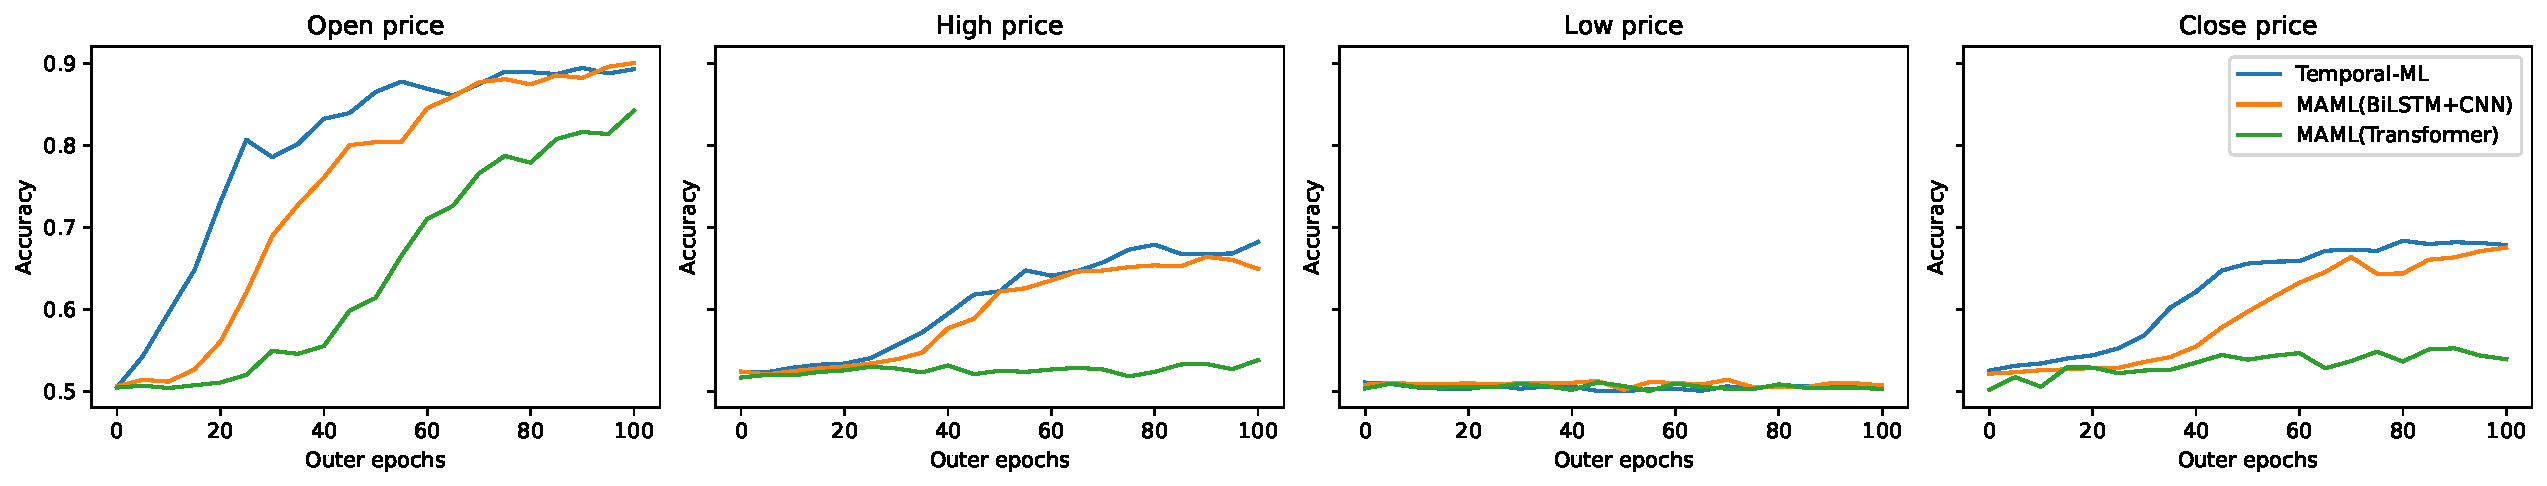
\includegraphics[width=\textwidth]{ab_att_usd.pdf}
        \cprotect\caption{\verb|Temporal-ML| vs. Models without \verb|BiLSTM| on \verb|USD/JPY|.}
        \label{fig:ablation_att_usd}
    \end{subfigure}
    ~
    \begin{subfigure}[b]{\textwidth}
        \centering
        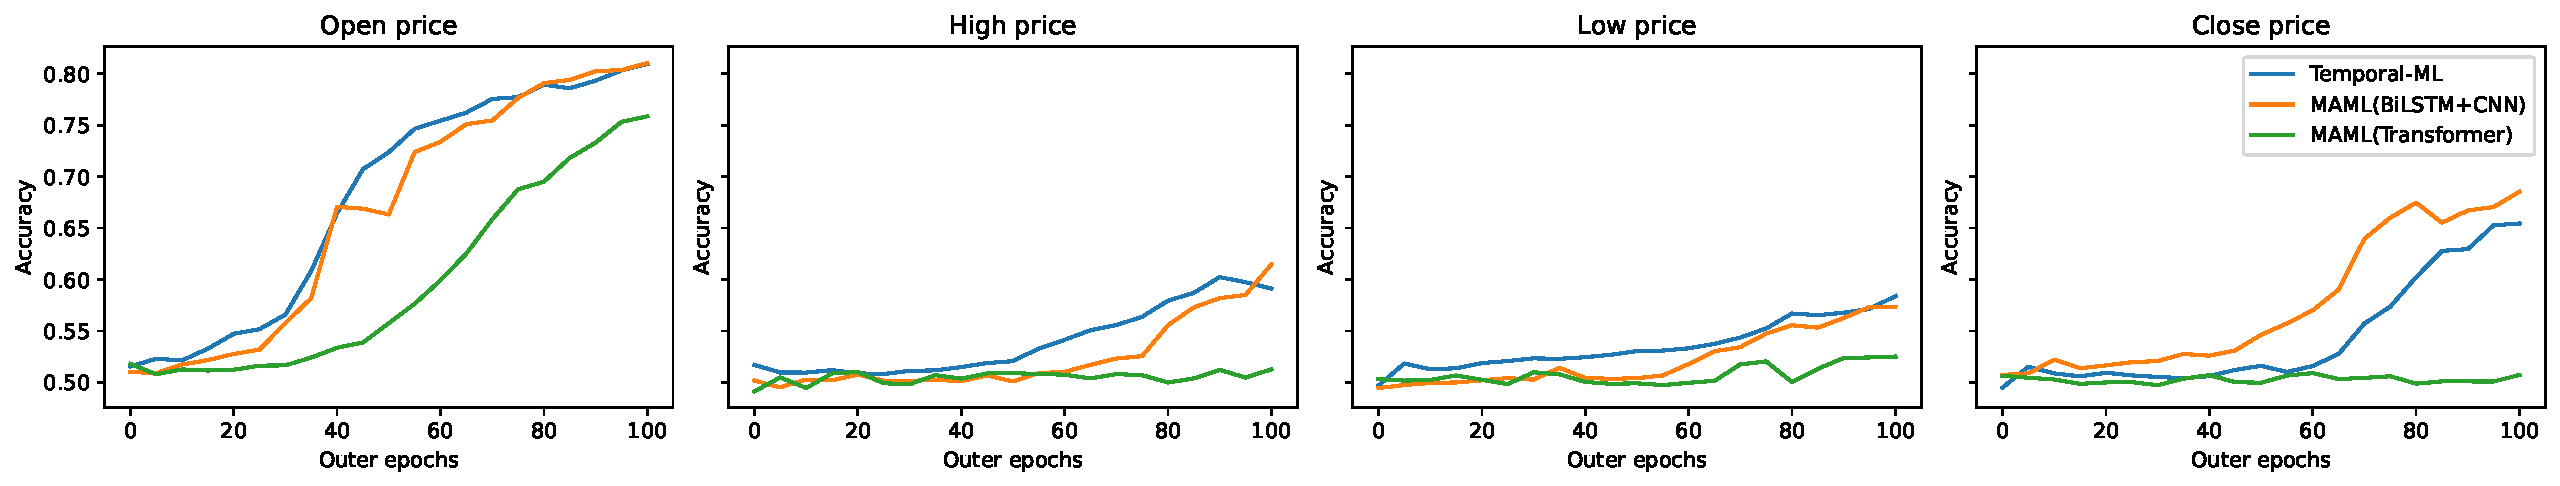
\includegraphics[width=\textwidth]{ab_att_multi.pdf}
        \cprotect\caption{\verb|Temporal-ML| vs. Models without \verb|BiLSTM| on \verb|multi-fx|.}
        \label{fig:ablation_att_multi}
    \end{subfigure}
    ~
    \begin{subfigure}[b]{\textwidth}
        \centering
        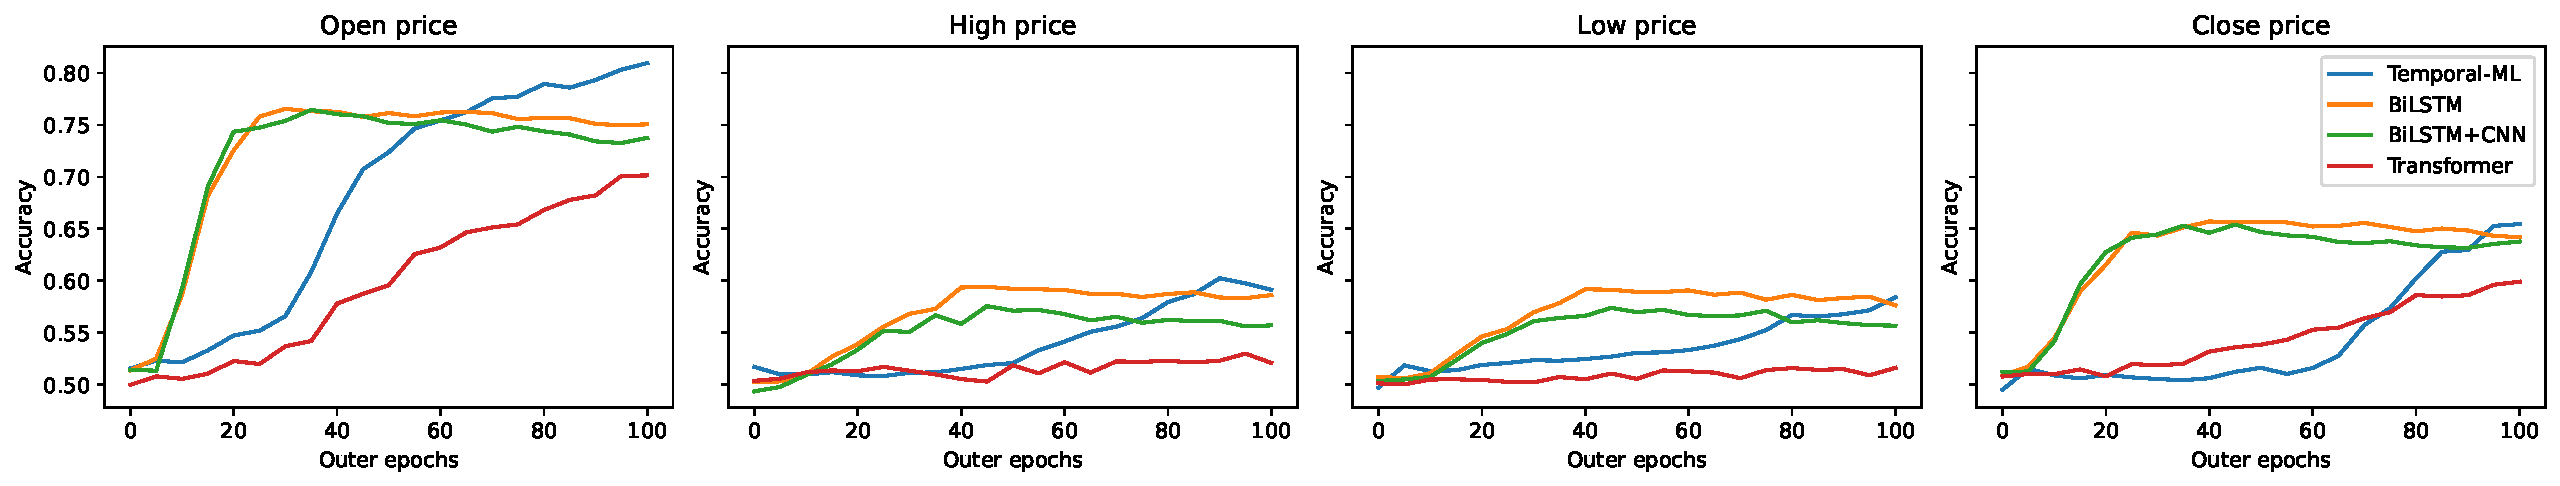
\includegraphics[width=\textwidth]{ab_ml_multi.pdf}
        \cprotect\caption{\verb|Temporal-ML| vs. Models without \verb|MAML| on \verb|multi-fx|.}
        \label{fig:ablation_ml_multi}
    \end{subfigure}
    \cprotect\caption{Convergence process of algorithms in ablation study on all attribute of foreign exchange datasets.}
    \label{fig:ablation}
\end{sidewaysfigure}

\section{Models' parameters aggregation ability}

% đấm nhits
% Trong quá trình tổng hợp các đặc trưng để đưa ra dự đoán cuối, \verb|NHITS| chỉ sử dụng các phép cộng trừ đơn giản. Điều này đặt trong ngữ cảnh của việc tổng hợp thông tin dựa trên các dải tần phân tách được từ dữ liệu đầu vào là hợp lý. Thật vậy, các dữ liệu liên quan đến thời tiết, nhu cầu sử dụng máy bay hoặc điện thể hiện tính chu kỳ rất mạnh vì thời tiết và hành vi tiêu dùng của con người, dù có thể chênh lệch theo thời gian nhưng vẫn thể hiện rất rõ tính mùa vụ (e.g., trời lạnh vào mùa đông, nhu cầu sử dụng máy bay tăng cao vào ngày lễ). Do đó, tần suất của loại dữ liệu này là một đặc trưng tốt và dễ dàng rút trích. Sau khi phân rã dữ liệu đầu vào thành các dải tần, chỉ cần tổng hợp chúng để có thể dự đoán tương lai. Ngoài ra, việc tổng hợp các dải tần bằng phép cộng đơn thuần có thể coi là rất đơn giản so với các thuật toán học sâu hiện tại, vốn làm việc trên không gian đặc trưng ẩn của dữ liệu. Do đó, quá trình tổng hợp của \verb|NHITS| trên dữ liệu phi chu kỳ gặp rất nhiều khó khăn vì thông tin đầu vào cho quá trình tổng hợp không tốt và phương pháp tổng hợp không hiệu quả. Từ đây, có thể thấy rằng, aperiodic time-series data trở thành điểm yếu chí mạng cho \verb|NHITS| và các phương pháp dựa trên việc phân rã tần số nói chung.

In the process of synthesizing features to make the final prediction, \verb|NHITS| only uses simple addition and subtraction. This makes sense in the context of synthesizing information based on the frequency bands extracted from the input data. Indeed, data related to weather, demand for airplanes or electricity show very strong periodic characteristics because weather and human consumption behavior, although they may vary over time, still show a very clear seasonality (e.g., cold weather in winter, high demand for airplanes during holidays). Therefore, the frequency of this type of data is a good feature and can be easily extracted. After decomposing the input data into frequency bands, we can simply synthesize them to be able to predict the future. In addition, synthesizing the frequency bands by an addition can be considered very simple compared to current deep learning algorithms, which work on the hidden feature space of the data. Therefore, the synthesis process of \verb|NHITS| on aperiodic data encounters many difficulties because the input information for the process is not good and the synthesis method is ineffective. Consequently, it can be seen that aperiodic time-series data becomes a fatal weakness for \verb|NHITS| and frequency decomposition-based methods in general.

% nâng bi bản thân
% Đối diện với sự phức tạp trong dữ liệu phi chu kỳ đòi hỏi một cấu trúc phức tạp để có thể tổng hợp các đặc trưng một cách hợp hiệu quả. Như đã đề cập trong phần Motivation (section \ref{sec:moti}), việc phân tích và tổng hợp thông tin từ nhiều nguồn dữ liệu trong cùng một domain có thể cung cấp các thông tin hữu ích trong việc dự đoán các chỉ số quan tâm. \verb|Temporal-ML| với khả năng tổng hợp thông tin dựa trên quá trình tối ưu của các thuật toán ML, cho phép mô hình nắm bắt thông tin đa chiều từ các nguồn dữ liệu khác nhau. Từ đó đưa ra dự đoán hiệu quả.

Dealing with the complexity of non-periodic data requires a complex structure that can efficiently aggregate features. As mentioned in the Motivation section (section \ref{sec:moti}), analyzing and synthesizing information from multiple data sources in the same domain can provide useful information for predicting metrics of interest. \verb|Temporal-ML| with the ability to synthesize information based on the optimization process of ML algorithms, allows the model to capture multi-dimensional information from different data sources. which helps produce effective predictions.

% phân tích bảng kq
% Để nắm bắt rõ khả năng của các thuật toán ML trong \verb|Temporal-ML|, chúng tôi loại bỏ component này khỏi thuật toán đề xuất sau đó chạy thực nghiệm để so sánh với kết quả ban đầu (subsection \ref{subsec:ablation_ml}). Chúng tôi sử dụng các thuật toán ML nhằm mục đích tổng hợp thông tin đa nguồn. Do đó, các so sánh chỉ được thực hiện trên tập dữ liệu \verb|multi-fx| vì chỉ tập dữ liệu này chứa nhiều tập dữ liệu con từ nhiều nguồn khác nhau. Kết quả được tổng hợp trong bảng \ref{tab:ab_ml}. Theo đó, với khả năng tổng hợp thông tin của mình, \verb|Temporal-ML| cho kết quả cao hơn từ 2-12\% so với các thuật toán không sử dụng ML trong quá trình huấn luyện. Ngoài ra, mức phân tán của các metrics cũng thấp hơn từ 1-7\%, chứng tỏ rằng mức chênh lệch trong quá trình dự đoán các task tốt hơn nhiều so với các thuật toán còn lại.

To evaluate the capabilities of ML algorithms in \verb|Temporal-ML|, we remove this component from the proposed algorithm and then run experiments to compare with the original results (subsection \ref{subsec:ablation_ml}). We use ML algorithms for the purpose of synthesizing multi-source information. Therefore, comparisons are only performed on the \verb|multi-fx| dataset because this dataset contains many sub-datasets from many different sources, which helps to accurately evaluate the information synthesis capability. The results are summarized in table \ref{tab:ab_ml}. Accordingly, with the information synthesis capability, \verb|Temporal-ML| achieves 2-12\% higher in all metrics than algorithms that do not use ML in testing process. In addition, the dispersion of the metrics is also lower from 1-7\%, proving that the difference in the task prediction process is much better than the remaining algorithms.

% Việc đạt được kết quả tốt hơn trên \verb|multi-fx| của \verb|Temporal-ML| là hoàn toàn dễ hiểu vì tất cả phương pháp còn lại trong bảng \ref{tab:ab_ml} đều không có khả năng tổng hợp thông tin như thuật toán đề xuất mà chỉ dựa hoàn toàn vào dữ liệu quá khứ để dự đoán tương lai. Do đó, không chỉ \verb|BiLSTM|, \verb|BiLSTM+CNN| mà ngay cả \verb|Transformer| cũng không thể tận dụng được mối tương quan giữa các data sources.

The better performance of \verb|Temporal-ML| on \verb|multi-fx| is understandable because all the remaining methods in the \ref{tab:ab_ml} table do not have the ability to synthesize information like the proposed algorithm, but rely entirely on past data to predict the future. Therefore, not only \verb|BiLSTM|, \verb|BiLSTM+CNN| but also \verb|Transformer| cannot take advantage of the correlation between data sources.

\begin{table}[H]
    \centering
    \cprotect\caption{Classification results (\%) of \verb|Temporal-ML| and models without \verb|MAML| on \verb|multi-fx|. Best results per metrics are boldfaced. (\mbox{*}): Our method.}
    \label{tab:ab_ml}
    \begin{tabular}{c|cccc} 
    \toprule
                                & $accuracy$              & $precision$             & $recall$                & $F1-score$                \\ 
    \hline
    \Verb|Temporal-ML|\mbox{*}  & $\mathbf{66.26\pm7.45}$ & $\mathbf{67.08\pm8.97}$ & $\mathbf{65.76\pm7.79}$ & $\mathbf{64.06\pm10.00}$  \\
    \Verb|BiLSTM|               & $63.88\pm9.00$          & $64.18\pm13.39$         & $63.66\pm9.13$          & $60.07\pm13.09$           \\
    \Verb|BiLSTM+CNN|           & $62.23\pm8.63$          & $62.89\pm9.76$          & $62.20\pm8.34$          & $59.91\pm10.97$           \\
    \Verb|Transformers|         & $58.44\pm9.15$          & $56.71\pm15.10$         & $58.22\pm8.84$          & $52.22\pm13.12$           \\
    \bottomrule
    \end{tabular}
\end{table}

% phân tích hội tụ
% Quá trình hội tụ của \verb|Temporal-ML| và các model without ML được trình bày trong hình \ref{fig:ablation_ml_multi}. Trong đó, khi dự đoán \textit{open price}, thuật toán đề xuất cho khả năng hội tụ vượt trội so với các thuật toán còn lại. Đối với các thuộc tính \textit{high price} và \textit{close price}, \verb|Temporal-ML| tỏ ra đuối sức trong giai đoạn đầu của quá trình huấn luyện. Tuy nhiên, khi về cuối, mô hình đề xuất cho thấy khả năng vượt lên nhanh chóng và tiềm năng cải thiện độ chính xác hơn nữa so với các thuật toán khác, vốn đã hội tụ.

The convergence of \verb|Temporal-ML| and the models without ML is shown in Fig. \ref{fig:ablation_ml_multi}. In particular, when predicting \textit{open price}, the proposed algorithm shows superior convergence compared to the remaining algorithms. For the attributes \textit{high price} and \textit{close price}, \verb|Temporal-ML| shows signs of slowing down in the early stages of training. However, towards the end, the proposed model shows the ability to quickly surpass and has the potential to further improve the accuracy compared to the other algorithms, which have already converged.

% Do đó, có thể thấy rằng, \textbf{việc sử dụng các thuật toán optimization-based ML trong việc tổng hợp thông tin là hoàn toàn hợp lý vì đã tận dụng thành công mối tương quan giữa các tập dữ liệu và đạt được độ chính xác cao mà không đòi hỏi quá nhiều dữ liệu như trong ngữ cảnh đơn nguồn}.

Therefore, it can be seen that, \textbf{the use of optimization-based ML algorithms in information synthesis is completely reasonable because it successfully takes advantage of the correlation between data sets and achieves high accuracy without requiring too much data as in the single-source context}.
